\chapter{Comparison of Different Algorithms}

% Do a good job of explain PSNR via this paper: https://en.wikipedia.org/wiki/Peak_signal-to-noise_ratio, or just ignore these values if  time does not hold

% Did we even run Huang's algorithm correctly?

We compare the performance of the three different algorithms used in this report by running the ray optics simulation. For Huang's algorithm, we consider both a viewing angle of 0 degrees and multiple viewing angles from -5 to 5 degrees in 1 degree increments. We also test the performance of the forward method and backward method on different angular resolutions (3x3 pinhole/lenlet vs 5x5 pinhole/lenslet). Potential advantages of the 3x3 pinhole or lenslet include improved resolution. However, the 3x3 pinhole filters out less light than the 5x5 pinhole, which can lead to more blurring. 

For all simulations, we use a screen size of 640x640 pixels, an object distance of 250 mm, and a focus distance of 380 mm. We use a depth of 6 mm for all algorithms except for the backward method with the pinhole mask (still use depth 6 mm for the backward method with the lens array) which uses a depth of 9 mm. The backwards method for the pinhole mask yields poor results at a depth of 6 mm because the prefiltering algorithm ignores too many pixels around the center pixel of the 3x3 or 5x5 superpixel. Thus, the prefiltered image is a bit dark, and the simulation is distorted by grided shapes. A larger depth will enable more screen pixels to pass through the pinhole because the angle of the ray traveling from the pixel to center of the closest pinhole is smaller. The metrics used to evaluate are contrast loss and RMSE from the chapter 8 as well as a new metric, peak signal-to-noise ratio.

\section{PSNR}

PSNR, or peak signal-to-noise ratio, measured in decibels, is used as a image quality measurement between an original and a compressed image. It is a ratio between the maximum power of a signal and the corrupting noise. The higher the value of PSNR, the better the quality of the compressed or reconstructed image.

We first define the mean square error ($MSE$), which is the cumulative squared error between the original image and the reconstructed image. Let $I_1$ and $I_2$ be the two images and $M$ and $N$ be the dimensions of $I_1$ and $I_2$, respectively.

$$MSE = \frac{\sum_{M,N}[I_1(m,n) - I_2(m,n)]^2}{M * N}$$

Let $R$ be the maximum fluctuation in the input image data, or difference between the largest possible value and smallest possible value. For example, in the RGB image where each channel is between 0 and 255, $R$ is 255. PSNR is computed by the following equation \cite{PSNR}.

$$PSNR = 10 log_{10} \left(\frac{R^2}{MSE}\right)$$

\section{Results}

Below are a copy of the original image and a blurred image, for reference.

\begin{table}[!h]
  \centering
    \caption{Original Images for Reference}
    \begin{tabular}{| c | c |}
    \hline Bunny Image & Word Image \\ \hline
      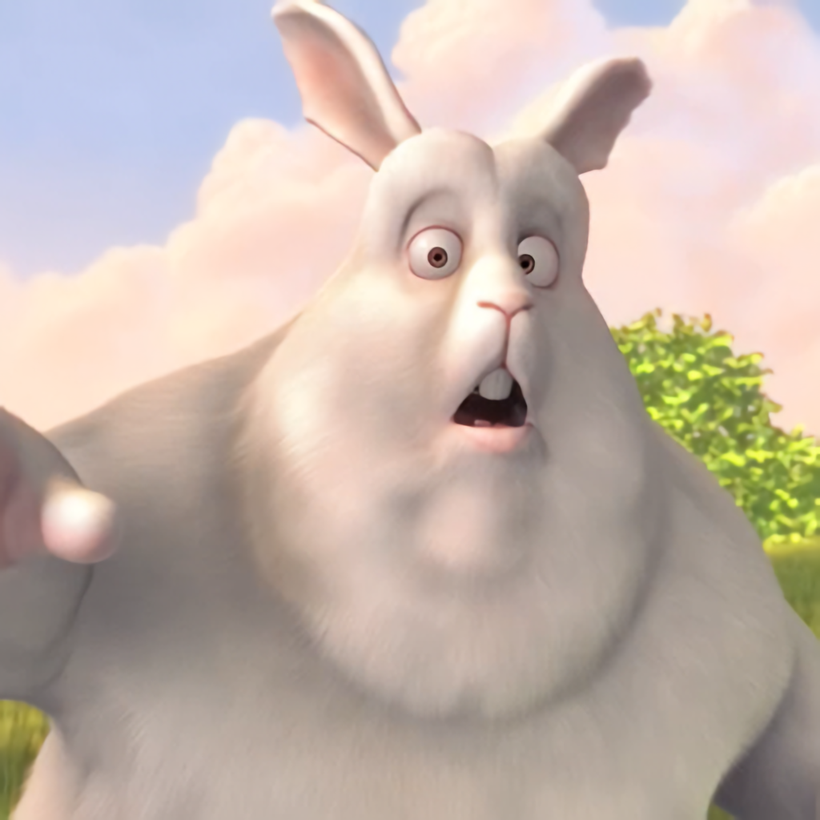
\includegraphics[width=2.5in]{chapters/chapter9/images/reference_image/origin.png} &
      
\includegraphics[width=2.5in]{chapters/chapter9/images/reference_image/origin_blur_image.png} \\ \hline
    \end{tabular}
\end{table}

The results are displayed in the next three pages.

\begin{table}[]
  \centering
     \caption{Huang's Algorithm and Forward Method}
    \begin{tabular}{| p{4 cm} | p{4cm} | p{4cm} | p{4cm} |}
    \hline Algorithm & Prefiltered Image & Pinhole Mask Simulation & Lens Array Simulation \\
    \hline Huang's Algorithm at One Angle & 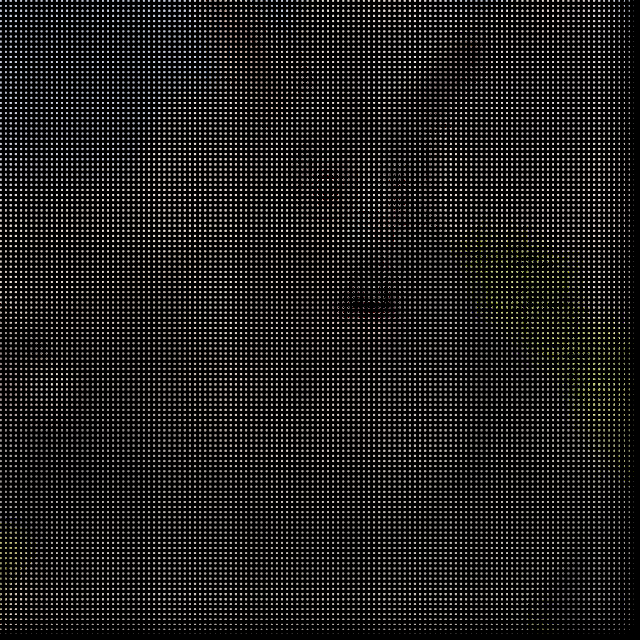
\includegraphics[width = 4 cm]{chapters/chapter9/images/simulation/Huang_1angle_prefilter.png} &
         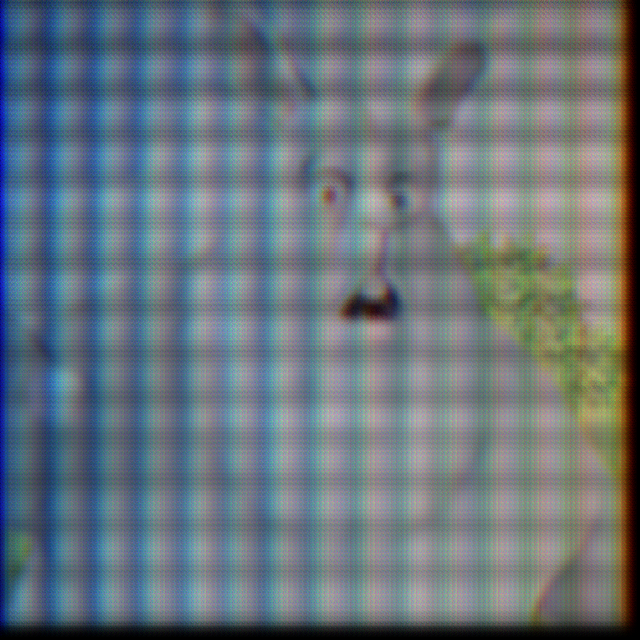
\includegraphics[width = 4 cm]{chapters/chapter9/images/simulation/Huang_1angle_pinhole_simulation.png} &  
         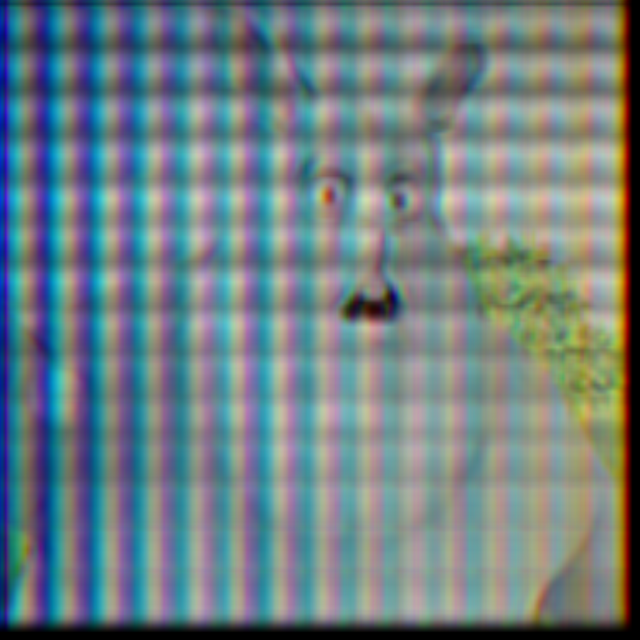
\includegraphics[width = 4 cm]{chapters/chapter9/images/simulation/Huang_1angle_lens_simulation.png} \\
    \hline Huang's Algorithm at Multiple Angles & 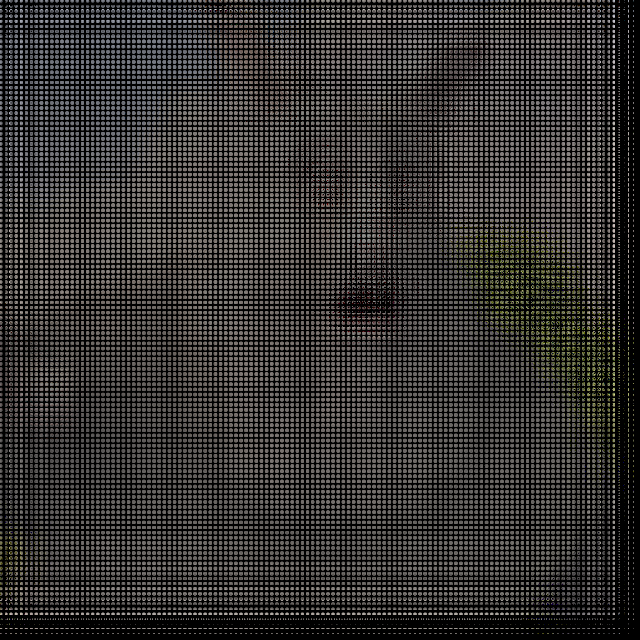
\includegraphics[width = 4 cm]{chapters/chapter9/images/simulation/Huang_allangle_prefilter.png} &
         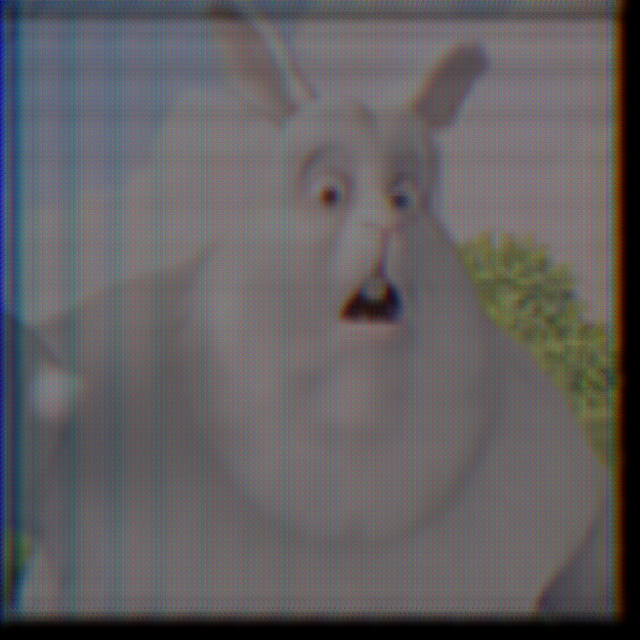
\includegraphics[width = 4 cm]{chapters/chapter9/images/simulation/Huang_allangle_pinhole_simulation.png} &  
         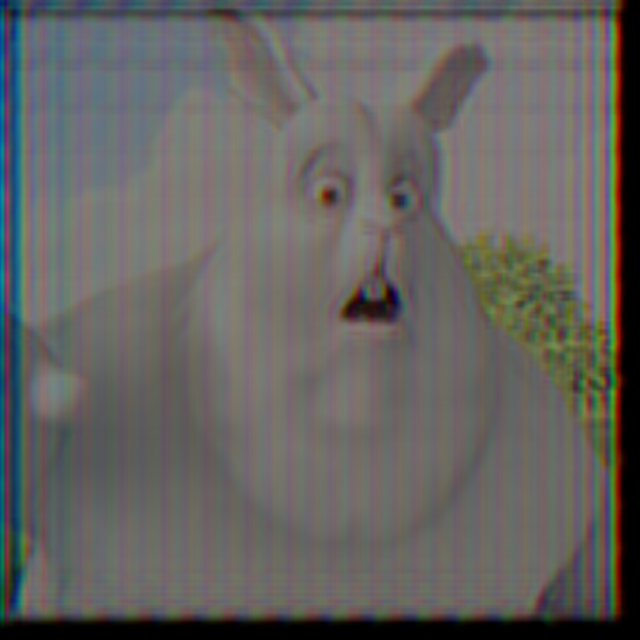
\includegraphics[width = 4 cm]{chapters/chapter9/images/simulation/Huang_allangle_lens_simulation.png} \\
    \hline Forward Method with 5x5 superpixel& 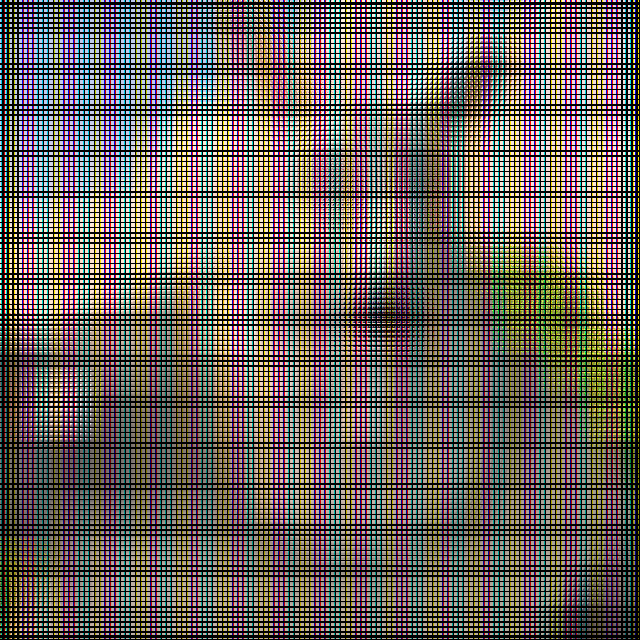
\includegraphics[width = 4 cm]{chapters/chapter9/images/simulation/5x5_prefilter.png} &
         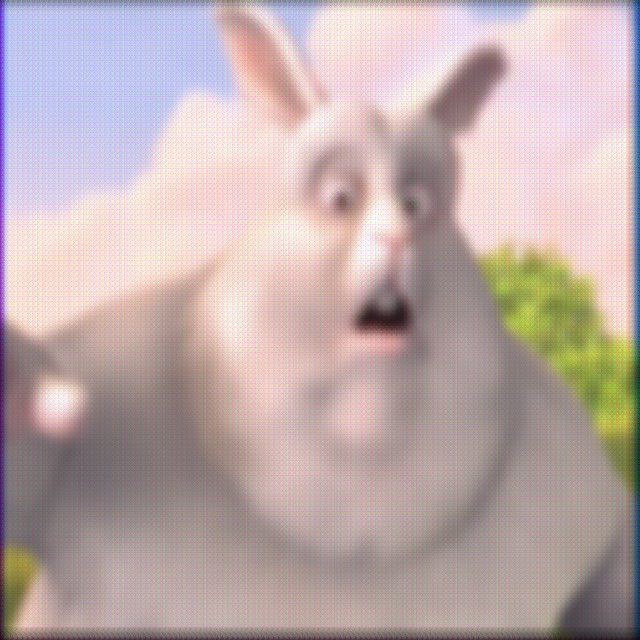
\includegraphics[width = 4 cm]{chapters/chapter9/images/simulation/5x5_pinhole_simulation.png} &  
         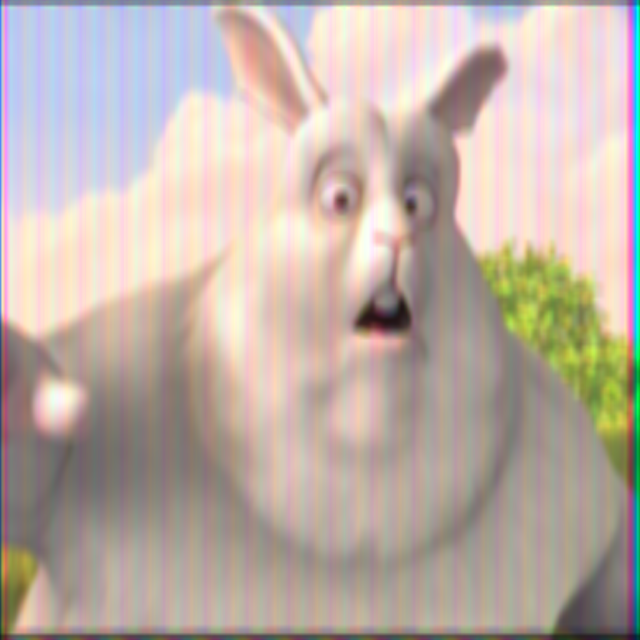
\includegraphics[width = 4 cm]{chapters/chapter9/images/simulation/5x5_lens_simulation.png} \\
    \hline Forward Method with 3x3 superpixel & 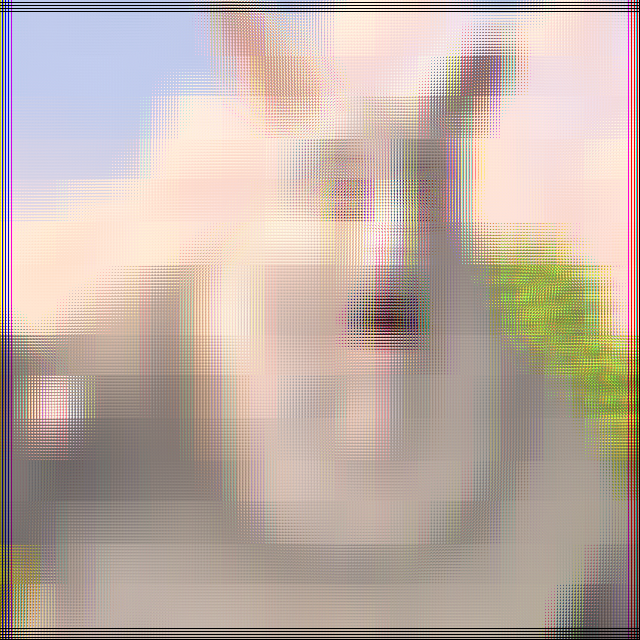
\includegraphics[width = 4 cm]{chapters/chapter9/images/simulation/3x3_prefilter.png} &
         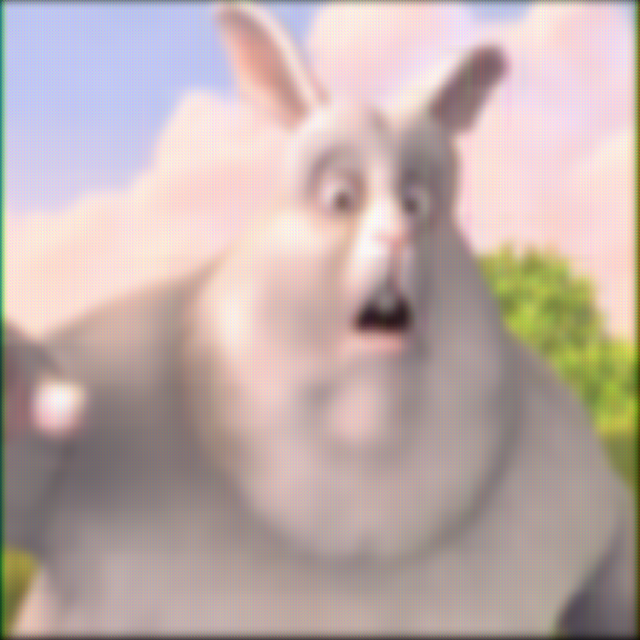
\includegraphics[width = 4 cm]{chapters/chapter9/images/simulation/3x3_pinhole_simulation.png} &  
         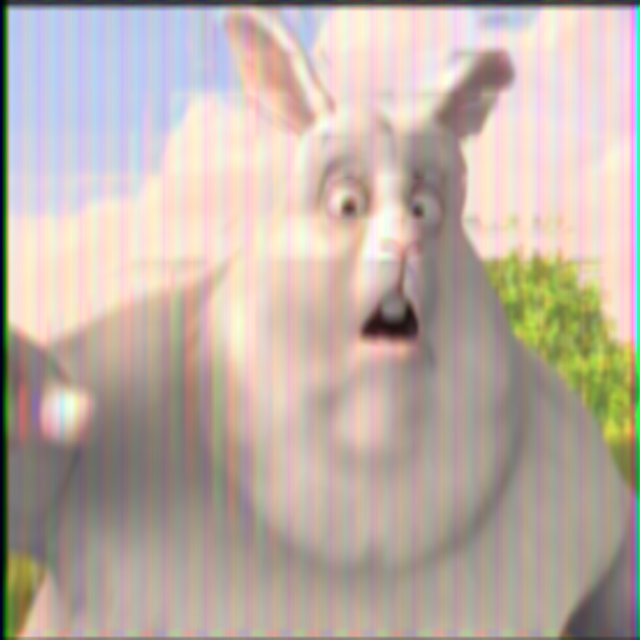
\includegraphics[width = 4 cm]{chapters/chapter9/images/simulation/3x3_lens_simulation.png} \\ \hline
  \end{tabular}
\end{table}

\begin{table}[]
  \centering
     \caption{Backward Method}
    \begin{tabular}{| p{5 cm} | p{4cm} | p{4cm}  |}
    \hline Algorithm & Prefiltered Image & Simulation \\
    \hline Backward Method for 5x5 Pinhole Mask & 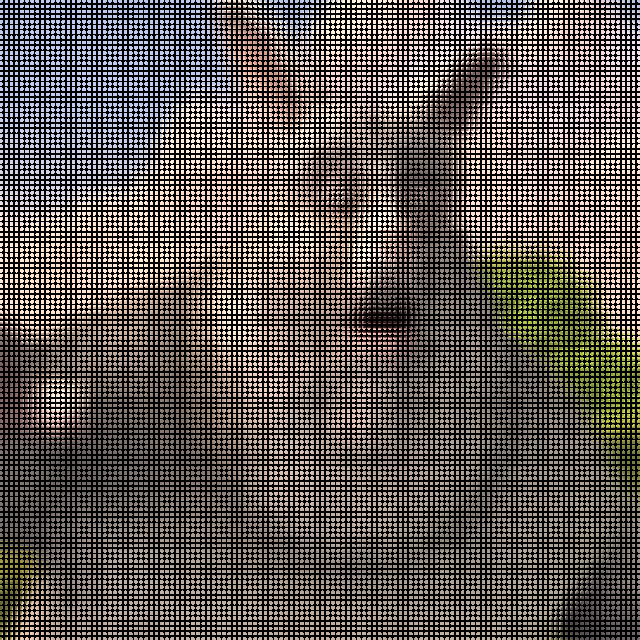
\includegraphics[width = 4 cm]{chapters/chapter9/images/simulation_backward/pinhole/prefilterResult_5x5_pinhole_depth9.png} &
        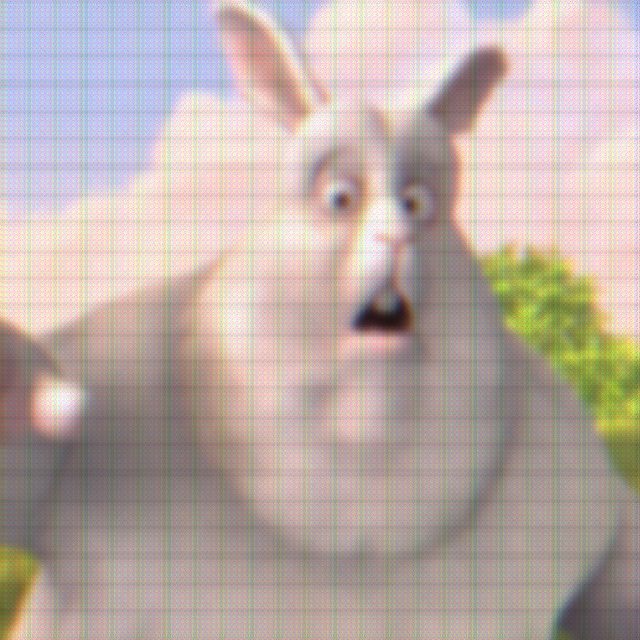
\includegraphics[width = 4 cm]{chapters/chapter9/images/simulation_backward/pinhole/simulationResult_5x5_pinhole_depth9.png} \\
    \hline Backward Method for 5x5 Lens Array & 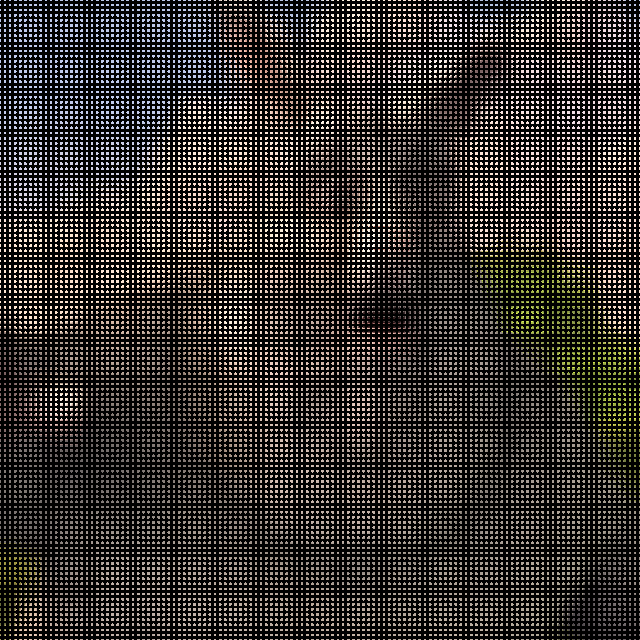
\includegraphics[width = 4 cm]{chapters/chapter9/images/simulation_backward/lens/prefilterResult_5x5_lens_depth6.png} &
        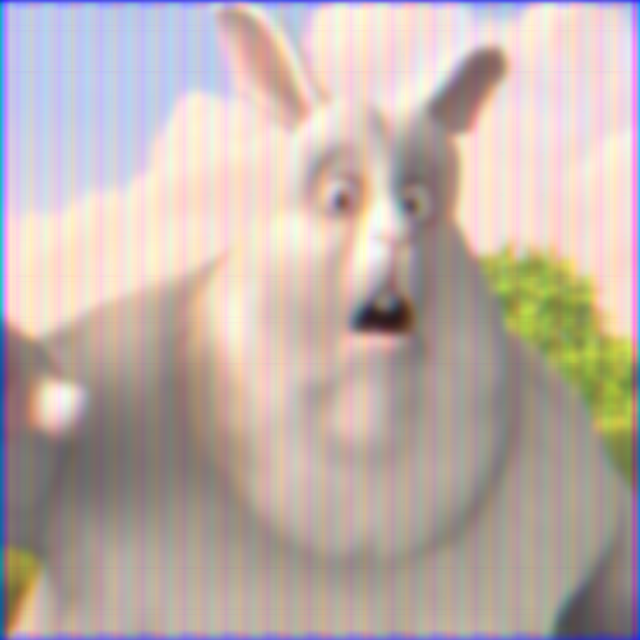
\includegraphics[width = 4 cm]{chapters/chapter9/images/simulation_backward/lens/simulationResult_5x5_lens_depth6.png} \\
    \hline Backward Method for 3x3 Pinhole Mask & 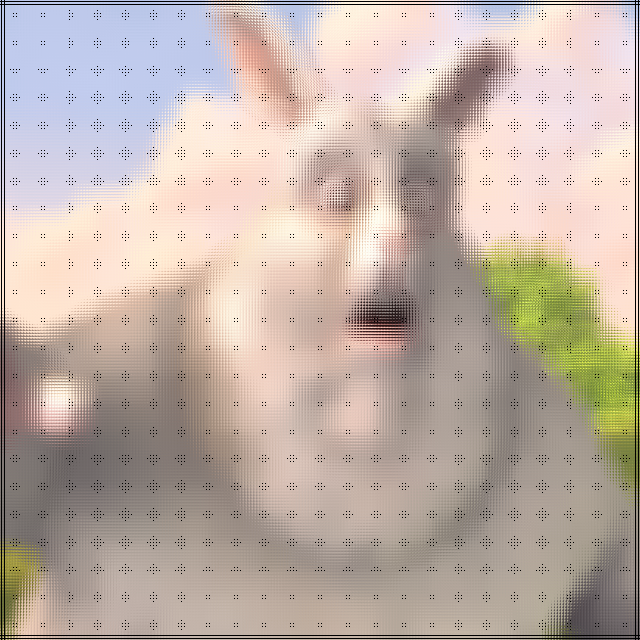
\includegraphics[width = 4 cm]{chapters/chapter9/images/simulation_backward/pinhole/prefilterResult_3x3_pinhole_depth9.png} &
        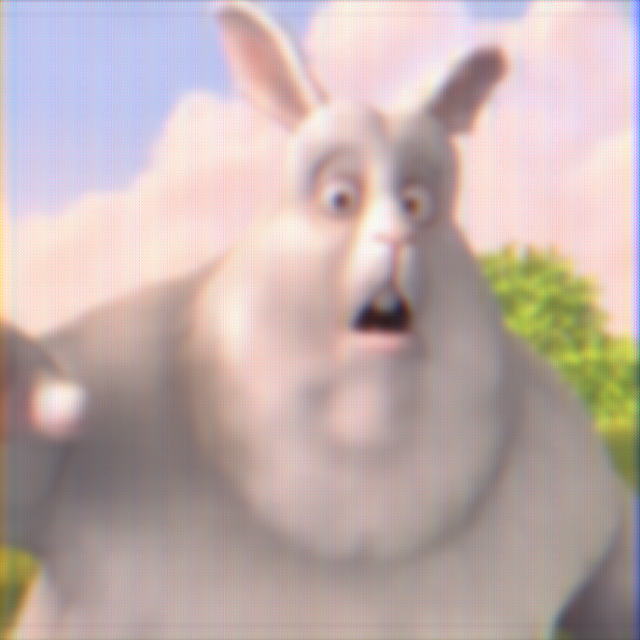
\includegraphics[width = 4 cm]{chapters/chapter9/images/simulation_backward/pinhole/simulationResult_3x3_pinhole_depth9.png} \\
   \hline Backward Method for 3x3 Lens Array & 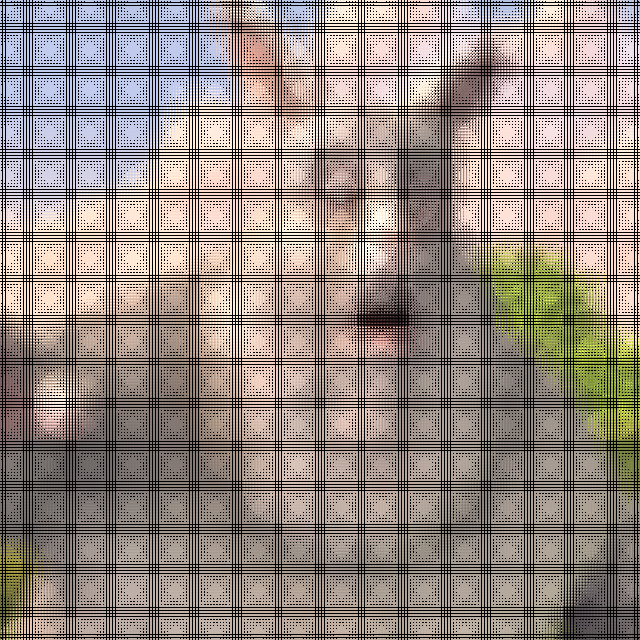
\includegraphics[width = 4 cm]{chapters/chapter9/images/simulation_backward/lens/prefilterResult_3x3_lens_depth6.png} &
        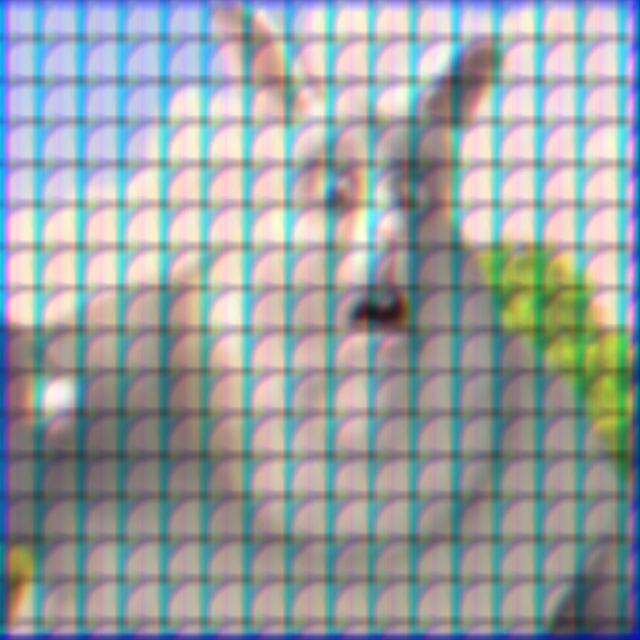
\includegraphics[width = 4 cm]{chapters/chapter9/images/simulation_backward/lens/simulationResult_3x3_lens_depth6.png} \\ \hline
  \end{tabular}
\end{table}

\begin{table}[]
  \centering
     \caption {PSNR}
    \begin{tabular}{| p{4 cm} | p{4 cm} | p{4cm} |}
    \hline Algorithm & Pinhole Mask & Lens Array \\
    \hline Huang's Algorithm at One Angle & 169.6088 & 170.1145 \\
    \hline Huang's Algorithm at All Angles & 167.6972 & 167.9586 \\
    \hline 5x5 Forward Method & 193.3367 & 195.9025 \\
    \hline 3x3 Forward Method & 197.2381 & 188.6442 \\ 
    \hline 5x5 Backward Method & 197.6123 & 198.9921 \\
    \hline 3x3 Backward Method & 203.575 & 181.2041 \\ \hline
    \end{tabular}
\end{table}

\begin{table}[]
  \centering
     \caption {RMSE}
     \begin{tabular}{| p{4 cm} | p{4 cm} | p{4cm} |}
    \hline Algorithm & Pinhole Mask & Lens Array \\
    \hline Huang's Algorithm at One Angle & 96197.46516 & 93412.11287 \\
    \hline Huang's Algorithm at All Angles & 107409.2307 & 105809.3705 \\
    \hline 5x5 Forward Method & 24449.74558 & 21083.34326 \\
    \hline 3x3 Forward Method & 19499.37489  & 32035.9960  \\ 
    \hline 5x5 Backward Method & 19162.62383 & 17592.97749 \\
    \hline 3x3 Backward Method & 13452.64547 & 49369.9328 \\ \hline
    \end{tabular}
\end{table}

\begin{table}[]
  \centering
     \caption {Contrast Loss}
     \begin{tabular}{| p{4 cm} | p{4 cm} | p{4cm} |}
    \hline Algorithm & Pinhole Mask & Lens Array \\
    \hline Huang's Algorithm at One Angle & 439806.6748 & 500561.2524 \\
    \hline Huang's Algorithm at All Angles & 526162.774 & 577569.688 \\
    \hline 5x5 Forward Method & 507178.0664 & 587265.172 \\
    \hline 3x3 Forward Method & 678130.4714  &  610534.7143 \\ 
    \hline 5x5 Backward Method & 372767.6833 & 646387.2938 \\
    \hline 3x3 Backward Method & 655407.2162 & 376476.1546 \\ \hline
    \end{tabular}
\end{table}

\section{Analysis}
Huang's algorithm at one angle yields a very dark prefiltered image. Many pixels appear to be blocked by the pinhole, and the non-black pixels have very small values, likely due to normalization by $n$ (see chapter 4). Huang's algorithm at multiple angles produces somewhat brighter prefiltered image, but still nowhere near that of the forward and backward methods. The pinhole mask simulation and the lens array simulation look very similar for Huang's algorithm at one angle and multiple angles. The darkness in the simulation leads to high RMSE, high mean squared error, and thus low PSNR. The bunny would be clear for Huang's algorithm at one angle if the grid was not blocking. Huang's algorithm for multiple angles produces the clearest bunny in terms of resolution.

The forward method yields moderately clear images with the pinhole mask display and very clear images with the lens array display with the exception of the RGB stripes. A 3x3 superpixel leads to more contrast loss than a 5x5 superpixel for both the pinhole mask and the lens array. In terms of both image quality or PSNR and image accuracy or RMSE, an angular resolution of 3 is better for the pinhole mask, and an angular resolution of 5 is better for the lens array. The forward method performs much better than Huang's algorithm in terms of both PSNR and RMSE due to the little amount of light lost, but the simulated images for Huang's algorithm at multiple angles have the clearest bunny features (eyes, nose, mouth, etc.).

The backward method produces images of highly varying quality due to the different depths chosen and therefore the prefiltering image that is produced. The 5x5 pinhole mask simulation shows a clear image with a grid outline of a few pixels that receive little light. The 3x3 pinhole mask simulation looks equally clear and has no pixels that receive little light. The 5x5 lens array produces an image similar to that of the forward method, but has slightly more severe RGB stripes.  The 3x3 lens array produces a completely distorted image. With the exception of the 3x3 lens array simulation, the backward method produces images with much higher PSNR and RMSE than Huang's algorithm and noticeably better RMSE and slightly better PSNR than the forward method. This shows that the backward method is able to retain more information about the original image than the two other algorithms. Finally, the 5x5 pinhole mask simulation yields the least amount of contrast loss out of all simulations, while the 3x3 pinhole mask and 5x5 lens array simulations have slightly higher contrast loss than the average forward method simulation.




